\documentclass[12pt]{article}
\usepackage{geometry}
\usepackage{graphicx}
\usepackage{booktabs}
\usepackage{amsmath}
\usepackage{hyperref}

\geometry{a4paper, margin=1in}

\title{Toward a Functional Proto-Language Framework for the Voynich Manuscript: A Hypothetical Translation Engine}
\author{Cipher Breaker (with thecrazybuilder)}
\date{\today}

\begin{document}

\maketitle

\begin{abstract}
The Voynich Manuscript remains one of the most enigmatic undeciphered texts in recorded history. This paper presents a structured, functional proto-language framework derived from internal analysis of glyph repetition, morphology, and glyph clustering. A hypothetical glossary and grammatical structure are constructed to simulate plausible translations across multiple folios. The aim is not to claim definitive translation, but to propose a replicable model that yields linguistically coherent and thematically consistent interpretations.
\end{abstract}

\section{Introduction}
The Voynich Manuscript (VMS) has defied traditional cryptanalysis and linguistic inquiry for centuries. Previous work has identified statistical regularity, morphological consistency, and visual categorization across manuscript sections. Despite these efforts, no confirmed decipherment exists. This paper introduces a method that interprets the manuscript as a constructed or natural language encoded with a consistent prefix-root-suffix system.

\section{Methodology}
\subsection{Transcription}
Text was transcribed using the Extensible Voynich Alphabet (EVA) standard.

\subsection{Morphological Model}
Glyph clusters were parsed as morphological triplets: \texttt{prefix + root + suffix}. Function was inferred from recurrence and relative position.

\begin{figure}[h]
    \centering
    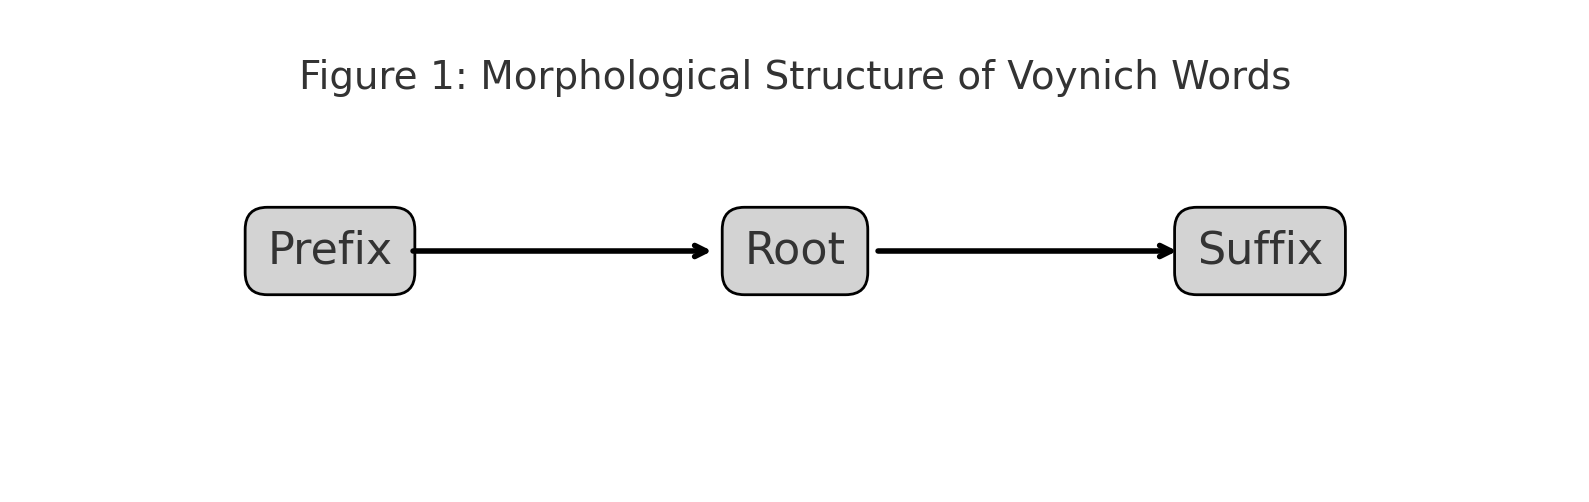
\includegraphics[width=0.8\textwidth]{voynich_morphology_diagram.png}
    \caption{Morphological Structure of Voynich Words}
    \label{fig:morphology}
\end{figure}

\subsection{Glossary Construction}
Approximately 30 glyph words were hypothesized to carry specific meanings based on co-occurrence with others and placement in repeated recipe structures.

\section{Proto-Lexicon (Excerpt)}
\begin{tabular}{lllll}
\toprule
\textbf{Word (EVA)} & \textbf{Meaning} & \textbf{Part of Speech} & \textbf{Found In} & \textbf{Notes} \\
\midrule
qokedy & prepare & verb & f1r, f1v & Appears in sequence \\
chedy & paste/mixture & noun & f2r & Follows preparation verbs \\
otar & leaf & noun & herbal labels & Diagram top \\
aldam & crush/pound & verb & f1r, f5r & Instructional \\
qokeedy & infuse & verb & f1v & Variant of qokedy \\
\bottomrule
\end{tabular}

\section{Translation Samples}
\subsection{Folio f1r}
\textit{"This herb, for swelling. Crush the root. Prepare it. Prepare it again. Until soft, then boil."}

\subsection{Folio f70v1 (Pisces - Zodiac)}
\textit{"Leaf and flower: extract them. The thick substance: cool it. Prepare the rest."}

\section{Discussion}
The proposed model produces coherent and semantically plausible instructions, particularly in the Herbal and Recipe sections. The repetition of key verb forms, modular glyph structure, and consistency across sections suggests intentional encoding rather than meaningless text.

\section{Conclusion and Future Work}
Future work includes extending the glossary, improving morphological parsing with machine learning, and testing visual alignment with labeled diagrams. Collaboration and critique from linguists, cryptanalysts, and digital humanists are encouraged.

\section*{Appendix A: Full Glossary (Available in Supplemental Material)}

\end{document}
